\section{Picard Iteration}
	\subsection{Lokale Lösung, Fortsetzung und Eindeutigkeit}
	Eine lokale Lösung von \eqref{eq:dgl_gew_allg} und entsprechenden ABs ist eine Lösung $y: I \to \R$ in einem offenen Intervall $x_0 \in I$, das beliebig klein sein kann, z.B.
	\begin{equation*}
		I = (x_0 - \varepsilon , x_0 + \varepsilon)
	\end{equation*}
	Sind $y: I \to \R$, $\tilde{y} : J \to \R$ zwei Lösungen des obigen AWPs und gilt weiterhin $ I \subset J$ und 
	\begin{equation}
		y(x) = \tilde{y}(x) \qquad , x \in I
	\end{equation}
	dann nennt man $\tilde{y}$ eine Fortsetzung der Lösung $y$.
	  \begin{figure}[H] 
		  \centering
		  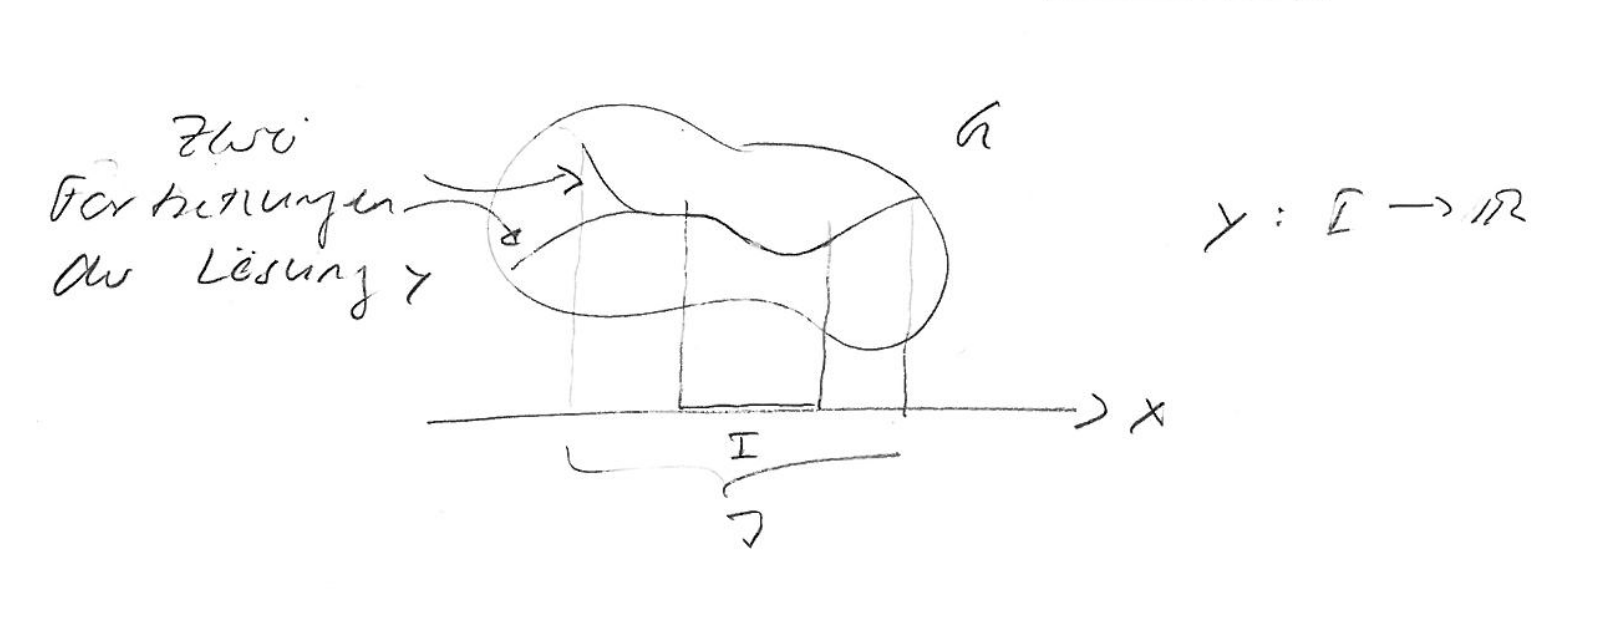
\includegraphics[width=0.9\textwidth]{./img/dgl_fortsetzung.png}
		  \caption{Fortgesetzte Lösungen von $y$}
		  \label{fig:dgl_fortsetz}
	  \end{figure}
	  
	  \begin{satz}
	  	Sind $f$ und $\partial_y f$ stetig auf dem Gebiet $G \subset \R^2$ und ist $(x_0, y_0) \in G$, dann hat das AWP 
	  	\begin{equation}
	  		y' = f(x,y) \qquad , y(x_0) = y_0
	  	\end{equation}
	  	genau eine Lösungskurve, die sich für $x < x_0$ und für $x > x0$ bis zum Rand von $G$ erstreckt. \newline
	  	Dass die Lösung von $y' = f(x,y), \; y(x_0) = y_0$ sich rechts von $x_0$ bis zum Rand von $G$ erstreckt bedeutet, dass
	  	\begin{equation}
	  		\Gamma+ = \lbrace (x,y(x))|x \geq x_0 \rbrace
	  	\end{equation}
	  	dem Rand $\partial G$ beliebig nahe kommt, oder unbeschränkt ist
	  \end{satz}
	
	
	\subsection{Satz von Picard-Lindelöf}
	\begin{satz}
		Für $x_0 \in \R,y_0 \in C^n,a,b>0$ setze 
		\begin{equation}
			I = [x_0 - a, x_0 +a]
		\end{equation}
		und 
		\begin{equation}
			Q = \lbrace \vec{z} \in \C^n | \max_{j=1,...,n} | z_j - <_{j_0} | \leq b \rbrace
		\end{equation}
		Ist die Funktion $F:I\times Q \to \C^n$ stetig, komponentenweise durch $R$ beschränkt und genügt sie bezüglich ihres 2. Arguments einer Lipschitz-Bedingung mit Lipschitz-Konstante $L$, so hat das AWP
		\begin{align}
			y'(x) = F(x,y(x))\\
			y(x_0) = y_0
		\end{align}
		auf dem Intervall $J=[x_0 - \alpha, x_0 + \alpha]$ mit $\alpha = \min \lbrace a, \frac{b}{R}\rbrace$ genau eine stetig differenzierbare Lösung $y:J \to Q$.  \label{ax:picard_lindeloef}
	\end{satz}
	\begin{bem}
		Da jedes DGL-System als System 1. Ordnung geschrieben werden kann, folgt aus obigem Satz, dass jedes AWP für ein DGL-System zumindest in einer kleineren Umgebung des AWs genau eine Lösung besitzt.
	\end{bem}
	\begin{bem}
		Genügsamkeit einer Lipschitz-Bedingung mit Lipschitz-Konstante $L$ wie in Satz \ref{ax:picard_lindeloef} gefordert bedeutet
		\begin{equation}
			|F_j(x,\vec{u}) - F_j(x,\vec{v})|\leq L \sum_{k=1}^n |u_k - v_k|	
		\end{equation}		 
	\end{bem}
	\begin{bsp}
		Es sei gegeben
		\begin{equation}
			y'(x) = \frac{x}{1-y(x)} \qquad \in (-1,1),\;y(0) = 0 \label{eq_pic_lind_bsp_a}
		\end{equation}
		und ist eine gewöhnliche DGL 1. Ordnung die durch Separation einfach lösbar ist.
		\begin{align*}
			&\Rightarrow y'(x) -y'(x) y(x) 0 x \Leftrightarrow \int y'(x) \dx - \int y'(x) y(x) \dx = \int x \dx \\
			&\text{mit }y(x) := u \Rightarrow du = y'(x)\dx \text{ folgt }\\
			&\Rightarrow y(x) - \int u \; du = \frac{1}{2} x^2 \Leftrightarrow y(x) - \frac{1}{2} y^2(x) = \frac{1}{2}x^2 + C \in \R \\
			&\Leftrightarrow y^2(x) - 2y(x) = -2\left(\frac{1}{2}x^2 + C\right) \Leftrightarrow 1-2y(x) + y^2(x) = 1-2\left(\frac{1}{2} x^2 +C\right) \\
			&\Leftrightarrow (y(x) - 1)^2 = 1-2\left(\frac{1}{2}x^2 + C\right) \Rightarrow y(x) = 1 \pm \sqrt{1-2\left(\frac{1}{2}x^2 + C\right)}\\
			&\Rightarrow y(x) = \pm \sqrt{1-x^2-2C}+1 \\
			&\Rightarrow y(0) = \pm \sqrt{1-2C}+1 \overset{!}{=} 0\Rightarrow 1=1-2C \Rightarrow C = 0 \\
			&\Rightarrow y(x) = 1 \pm \sqrt{1-x^2} \qquad, x \in (-1,1)
		\end{align*}
		Es gilt $I = [-a,a]$ und $Q = [-b,b]$. Weiterhin gilt nach \eqref{eq_pic_lind_bsp_a} und mit $y'(x) := F(x,y)$
		\begin{equation}
			F(x,y) = \frac{x}{1-y} \qquad für \; x \in I, y \in Q
		\end{equation}
		Durch die Wahl von $a$ und $b$ wird die Aussage des Satzes beeinflusst (Größe von $J$). Hier muss $b<1$ sein (wegen der Definition von F). Da wir die Lösung kennen, macht ein $\alpha \geq 1$ keinen Sinn. Somit ergibt sich
		\begin{equation}
			|F(x,y)| \leq \frac{a}{1-b} := R \qquad, x \in I, y \in Q
		\end{equation}
		Mit
		\begin{align}
			|F(x,y) - F(x,z)| &= \left| \frac{x}{1-y} - \frac{x}{1-z} \right| = |x| \left| \frac{1-z-(1-y)}{(1-y)(1-z)}\right| \nonumber \\
			&\leq \frac{a}{(1-b)^2} |y-z|
		\end{align}
		folgt Lipschitz-Stetigkeit bezüglich $y$ für alle $x \in I$ und alle $y,z \in q$. $\alpha$ ergibt sich somit zu 
		\begin{equation}
			\alpha = \min \lbrace a, \frac{b}{R} \rbrace = \min \lbrace a, \frac{b(1-b)}{a} \rbrace
		\end{equation}
	\end{bsp}
	
	\subsection{Näherung durch sukzessive Appproximation (Picard Iteration)}
	Die grundlegende Idee ist die Umformulierung des AWP durch eine Integration. Damit ergibt sich
	\begin{equation}
		y(x) = y_0 + \int_{x_0}^x f(\xi , y(\xi)) \;d\xi
	\end{equation}
	für alle $x \in J$, wobei $J$ das Intervall au dem Satz von Picard-Lindelöf (Satz \ref{ax:picard_lindeloef}) ist. \newline
	Beginnend mit einer konstanten Funktion
	\begin{equation}
		y_0(x) := y_0
	\end{equation}
	kann man durch Rekursion
	\begin{equation}
		y_k(x) = y_0 + \int_{x_0}^x F(\xi , y_{k-1}(\xi))\;d\xi \qquad x \in J, k \in \N
	\end{equation}
	eine  Folge von Funktionen definieren, die wir $(y_k)$ nennen. Diese Folge konvergiert gegen die Lösung des AWP, und zwar so, dass für die j-ten Komponenten von $y_k$ und $y$ gilt
	\begin{equation}
		\max_{y=1...n} \max_{x \in J} |y_{jk}(x) - y_j (x)| \to 0 \quad (k \to \infty) \label{eq:picard_iteration}
	\end{equation}
	$(y_k)$ heißt auch Folge der sukzessiven Approximation. Die Konvergenzaussage kann durch eine Abschätzung weiter konkretisiert werden.
	\begin{equation}
		\max_{j=1...n} \max_{x \in J} |y_{jk}(x) - y_j (x)| \leq \frac{(L n \alpha)^k}{k!}\cdot e^{L n \alpha} \cdot \max_{j=1...n} \max_{x \in J} |y_{j_1}(x) - y_{j_0} (x)|
	\end{equation}
	für alle $k \in \N_0$ mit den Konstanten $L$ und $\alpha$ aus dem Satz von Picard-Lindelöf (Satz \ref{ax:picard_lindeloef}). Man nennt diese Ungleichung A-Priori Abschätzung für die Güte der Approximation durch die Lösung der k-ten sukzessiven Approximation. Damit kann die Güte für alle Folgenglieder sofort abgeschätzt werden, solange  zumindest $y_0$ und $y_1$ bestimmt worden sind.
	\begin{bsp}
		Gegeben sei
		\begin{equation}
			u'(x) = x(u(x))^2 \qquad, u(0) = \frac{1}{2}
		\end{equation}
		Die DGL lässt sich zunächst leicht über einen Separationsansatz lösen.
		\begin{align*}
			&\frac{u'(x)}{u(x)^2} = x \Leftrightarrow \int \frac{u'(x)}{u(x)^2} \dx = \int x \dx \\
			&\text{mit } u(x) := s \Rightarrow ds = u' \dx \\
			&\Leftrightarrow \int \frac{1}{s^2} \;ds = - \frac{1}{s} = - \frac{1}{u(x)} = \frac{1}{2} x^2 + C_1 \\
			&\Rightarrow u(x) = - \frac{2}{x^2 + 2 C_1} = -\frac{2}{x^2 + C} \quad, C_1,C \in \R \\
			&\Rightarrow u(0) \overset{!}{=} \frac{1}{2} = - \frac{2}{C} \Rightarrow C = -4 \\
			&\Rightarrow u(x) = -\frac{2}{x^2 - 4} = \frac{2}{4-x^2}
		\end{align*}
		Damit ergibt sich für die Bestimmung der Konstanten
		\begin{align*}
			&\Rightarrow F(x,u) = xu^2 \qquad, x \in [-1,1], u \in [0,1] \\
			&\Rightarrow |F(x,u)| \leq 1 \\
			&\Rightarrow |F(x,u) - F(x,v)| \leq |x(u-v)(u+v)| \leq 2|u-v| \\
			&\Rightarrow a = 1,\; b = \frac{1}{2}, \; R = 1, \; L = 2 \Rightarrow \alpha = \frac{1}{2}\\
		\end{align*}
		Nun lässt sich die AB $u_0 = \frac{1}{2}$ in die Rekursionsvorschrift \eqref{eq:picard_iteration} einsetzen.
		\begin{align*}
			&\Rightarrow u_1(x) = \frac{1}{2} + \int_{0}^x t\left(\frac{1}{2}\right)^2 \;dt = \frac{1}{2} + \frac{1}{8 x^2}\\
			&\Rightarrow u_2(x) = \frac{1}{2} + \int_0^x t \left( \frac{1}{2} + \frac{1}{8}t^2\right)^2\;dt = \frac{1}{2} + \frac{1}{8}x^2 + \frac{1}{32}x^4 + \frac{1}{384}x^6\\
			&\dots
		\end{align*}
		So können weitere Werte berechnet werden. Mit den nun bekannten Größen kann direkt eine Abschätzung durchgeführt werden.
		\begin{align*}
			&\Rightarrow \max{x \in J} |u_1 (x) - u_0 (x)| = \max{x \in [-\frac{1}{2}, \frac{1}{2}]} \left| \frac{1}{2} + \frac{1}{8}x^2 - \frac{1}{2}\right| = \frac{1}{32} := (*) \\
			&\Rightarrow \frac{(L n k)^k}{k!}e^{L n k} = \frac{(2 \cdot 1 \cdot  \frac{1}{2})^1}{1} e^{2 \cdot 1 \cdot \frac{1}{2}} = e := (**) \\
			&\Rightarrow (*) \cdot (**) \approx 0,08494631
		\end{align*}
		$\Rightarrow$ Bei Polynomen als Ergebnis sind die Näherungen oft sehr schnell sehr gut.
	\end{bsp}